There are several overlapping clustering methods that include (e.g.~\cite{perez2013oclustr} and~\cite{bonchi2013overlapping}), which looks relevant for our framework. However these methods does not fit our purpose both equal-size  constraints for the local kernel machines. We also found them very slow in practice because their complexity varies from cubic to quadratic (with a big constant factor) on the training-set. These problems motivated us to propose a practical method that builds overlapping local kernel-machines with spatial and equal-size constraints. \ignore{Efficiently decomposing the domain with equal-size constraints is critical for our purpose. This is} These constraints are critical for our purpose since the number of points in each kernel-machine determine its local performance. Hence,  our training phase is two steps: (1) the training data is split into $K= N/ (1-p) M$ equal-sized clusters of $(1-p) M$ points. (2) an ODC with K overlapping subdomains is generated by augmenting each cluster with $p \cdot M$ points from the neighboring clusters.\ignore{ based on $M$ and $p$ and an ODC training model is learned by building a kernel machine on each subdomain.}
%\begin{figure}[t!]
%\centering
%    \begin{subfigure}[b]{0.20\textwidth}
%    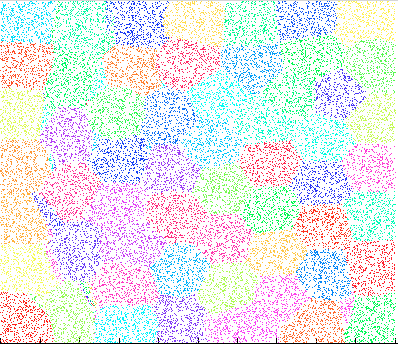
\includegraphics[width=1.0\textwidth,height=0.75\textwidth]{Ekmeans57.png}
%               \caption{$\,\,$}
%                \label{fig:ekmeans}
%        \end{subfigure}%
%        \begin{subfigure}[b]{0.22\textwidth}
%   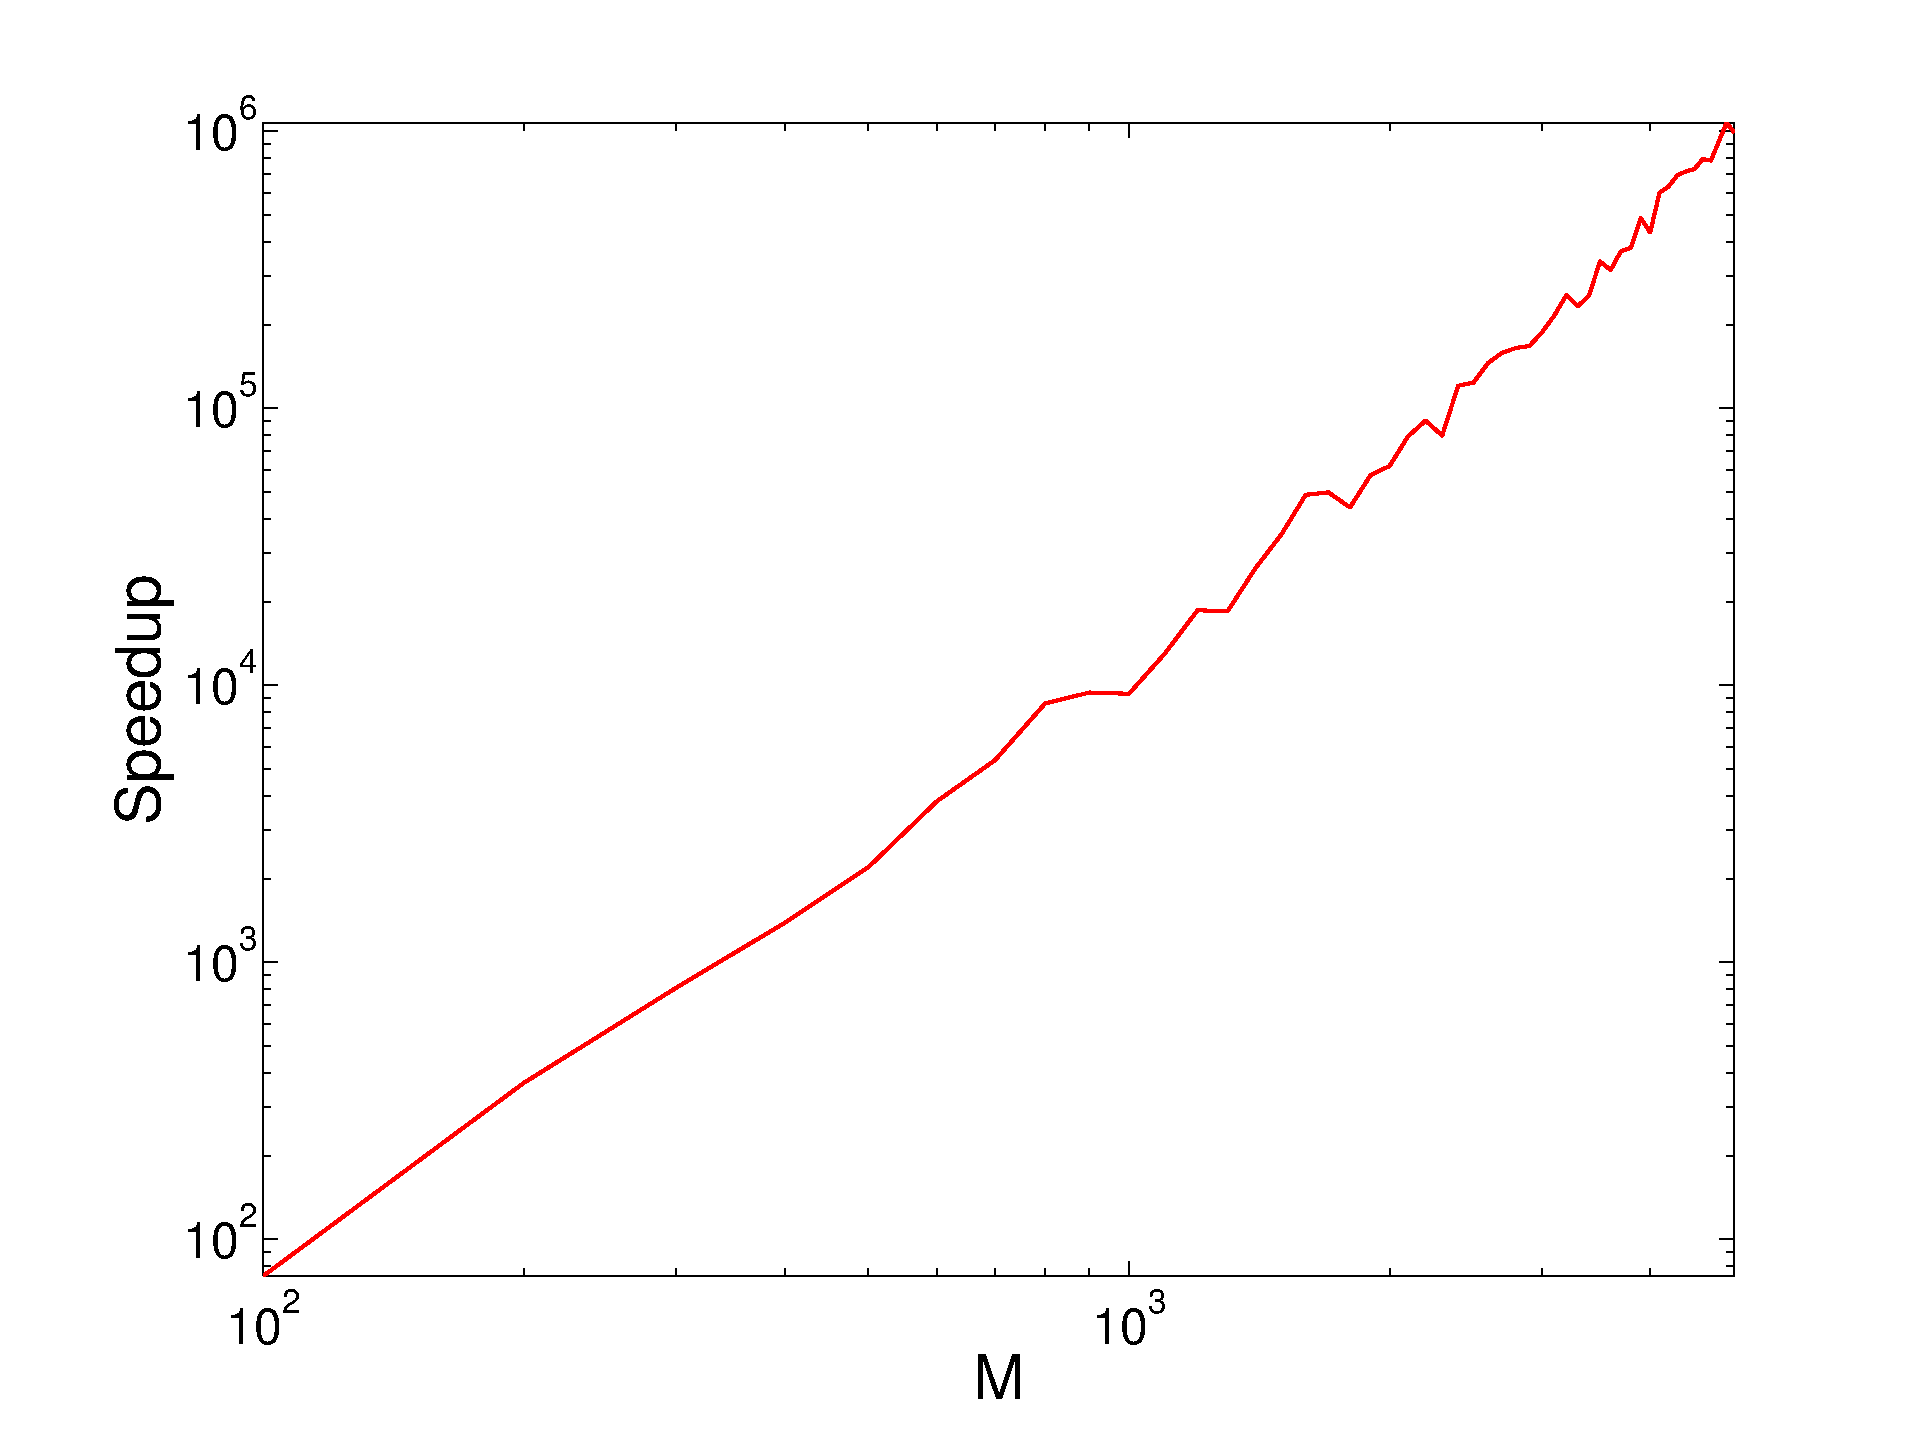
\includegraphics[width=1.0\textwidth,height=0.71\textwidth]{figMInvSpeedUp.eps}
%                \caption{$\,\,$}
%                 \label{fig:SpeedUp}
%        \end{subfigure}
%        \vspace{-4mm} 
%        \caption{(a) AB-EKmeans on 300,000 2D points, K= 57\ignore{ (best seen electronically)}(b) ODC-prediction speedup on either TGP or GPR for retrieving precomputed matrix inverses as $M$ increases, compared with computing them on test time by NN scheme (log-log scale)}
%\vspace{-4.5mm}        
%\end{figure}
%\begin{figure}
%\centering
%\begin{tabular}{cc}
%\bmvaHangBox{\fbox{
%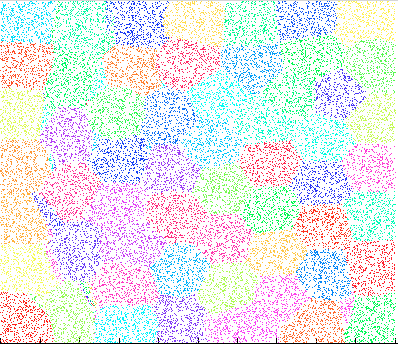
\includegraphics[width=2.8cm]{Ekmeans57.png}}}&
%\bmvaHangBox{\fbox{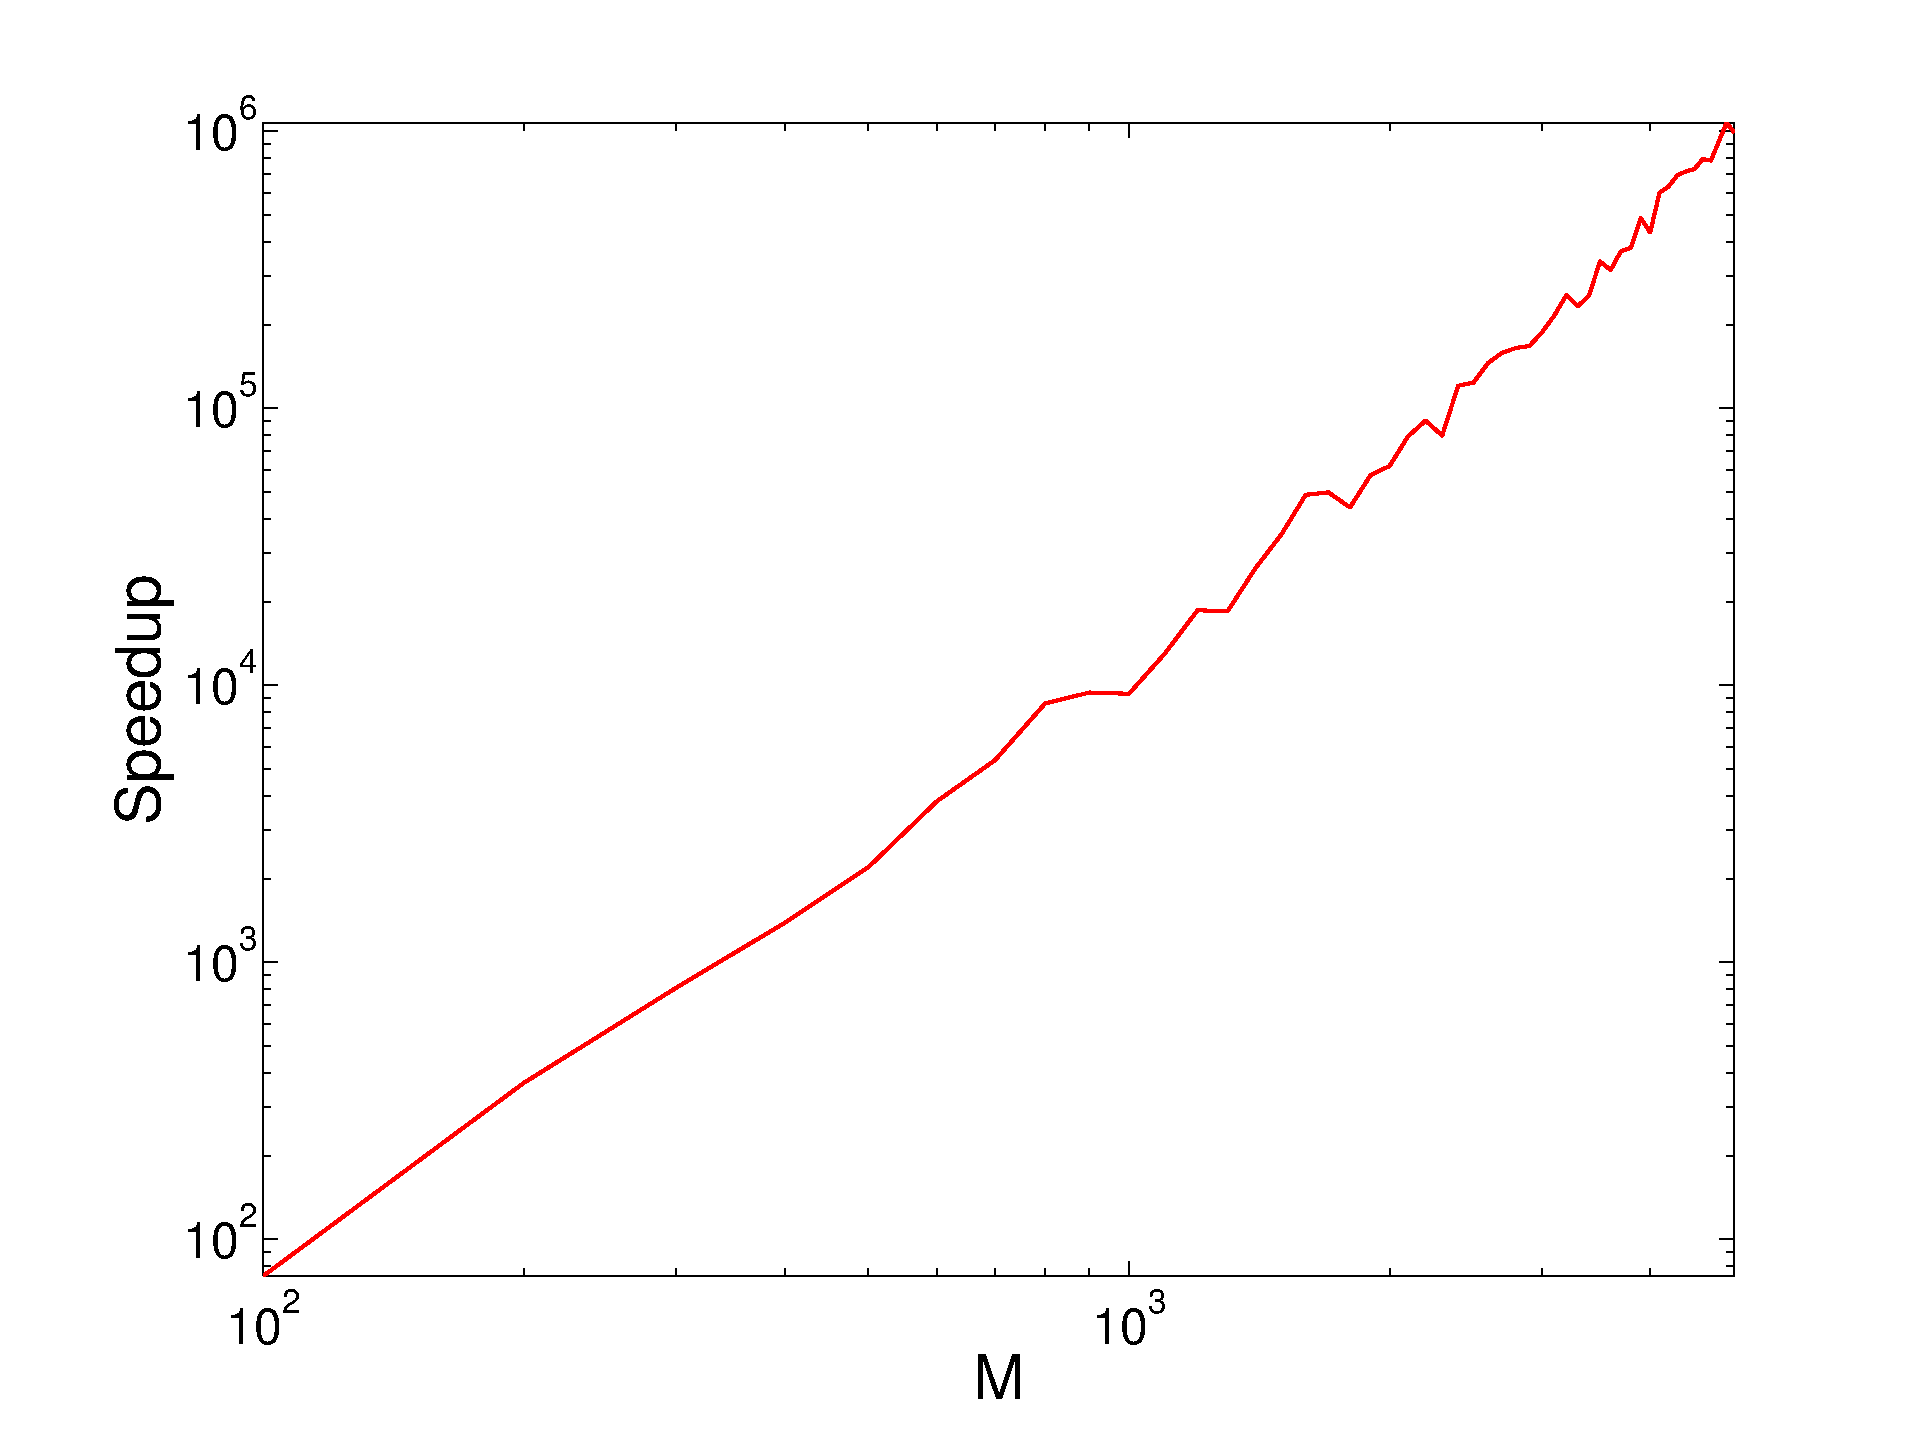
\includegraphics[width=2.8cm]{figMInvSpeedUp.eps}}}\\
%%\bmvaHangBox{\fbox{\includegraphics[width=5.6cm]{OverlappingFig.png}}}\\
%(a)&(b)
%\end{tabular}
%\caption{(a) AB-EKmeans on 300,000 2D points, K= 57\ignore{ (best seen electronically)}(b) ODC-prediction speedup on either TGP or GPR for retrieving precomputed matrix inverses as $M$ increases, compared with computing them on test time by NN scheme (log-log scale)}
%\label{fig:overlapandnonoverlap}
%\end{figure}

\vspace{-1.5mm}
\subsubsection{Equal-size Clustering}

\ignore{The performance of the local regression model depends on the number of points in each partition.
In order to bound the computation, we need the subdomains to be balanced in size. This is achieved by splitting the data into equal-sized clusters, and use these clusters to establish the subdomains. } There are recent algorithms that deal with size constraints in clustering. For example,\ignore{Zhu \etal}~\cite{Zhu2010} formulated the problem of clustering with size constraints as a linear programming problem. However such algorithms are not computationally efficient, especially for large scale datasets (e.g., Human3.6M). We study two efficient ways to generate equal size clusters; see Table~\ref{tab:thcomp} (last row) for their ODC-complexity.

\vspace{2mm}

\noindent \textbf{Recursive Projection Clustering (RPC) \cite{Chalupka:2013}.}
In this method,\ignore{\cite{Chalupka:2013} proposed to partition} the training data is partitioned to perform GPR prediction. \ignore{In summary, they begin with assigning } Initially all  data points are put in one cluster. Then, two points are chosen randomly\ignore{ to create a line through them.} and orthogonal projection of all the data onto the line connecting them is computed. Depending on the median value of the projections, The data is then split into two equal size subsets. The same process is then applied to each cluster to generate $2^l$ clusters after $l$ repetitions. The iterations stops once $2^l>K$. As indicated, the number of clusters in this method has to be a power of two and it might produce long thin clusters. 

\ignore{K-means clustering ~\cite{Hartigan1979} splits the domain such that the clusters have similar spatial extent, resulting in Voronoi partitioning.  However,  this is not what is needed for efficient computation of kernel machines.}

\ignore{
Therefore, we propose two greedy algorithms to obtained equal-size clustering. }

\vspace{2mm}

\noindent \textbf{Equal-Size K-means (EKmeans).} We propose a variant of k-means clustering~\cite{Hartigan1979} to generate equal-size clusters.\ignore{The algorithms mainly modify the assignment step of the k-means to bound the size of the resulting clusters.  }\ignore{Given a set of data points $X=\{\mathbf{x}_1, \cdots, \mathbf{x}_N  \}$, t} The goal is to obtain disjoint partitioning of $X$ into clusters $C=\{C_1, \cdots, C_K\}$,  similar to the k-means objective, minimizing the within-cluster sum of squared Euclidean distances, $ C = \arg_C J(C) = \min \sum_{j=1}^K \sum_{\mathbf{x_i}\in C_j} d(\mathbf{x_i}, \boldsymbol{\mu}_j)$,  
\ignore{\[ \small C = \arg_C \min \sum_{j=1}^K \sum_{\mathbf{x_i }\in C_j} d(\mathbf{x_i},\boldsymbol{\mu}_j) \]}
where $\boldsymbol{\mu}_i$ is the mean of cluster $C_i$, and $d(\cdot,\cdot)$ is the squared distance. Optimizing this objective is NP-hard and  k-means iterates between the assignment and update steps as a heuristic to achieve a solution; $l_1$ denotes number of iterations of kmeans. We add equal-size constraints  $\forall  (1 \leq i  \leq K),  |C_i| = N/K = (1-p) M$. \ignore{We add extra constraints to the problem to guarantee equal-sized partitioning $\forall  (1 \leq i  \leq K),  |C_i| = N/K$. }

\ignore{
In order to achieve this partitioning, we propose two heuristic algorithms, which mainly modify the assignment step of the k-means to bound the size of the resulting clusters. We introduce here one of them which achieves less cost $J(C)$; see SM for pseudo code of the two algorithms and our cost analysis of them. We call the better algorithm {\em Assign and Balance (AB) EKmeans}, in which }
\ignore{{\em (2) Iterative Minimum-Distance Assignments (IMDA) k-means:} we initialize a pool of unassigned points $\tilde{X}  =  X$ and initialize all clusters as empty.  Given the means computed from the previous update steps, we compute the distances $d(\mathbf{x}_i,\boldsymbol{\mu}_j)$ for all points/center pairs. We iteratively pick the minimum distance pair 
\[\small (\mathbf{x}_p,\mathbf{mu}_l)  : d(\mathbf{x}_p,\boldsymbol{\mu}_l) \le d(\mathbf{x}_i,\boldsymbol{\mu}_j)  \forall x_i \in \tilde{X} \text{and}  |C_l| < N/K \]
and assign point $x_p$ to cluster $l$. The point is then removed from the pool of unassigned points. if  $|C_l| = N/K$,  then it is marked as balanced and no longer considered. The process is repeated until the pool is empty.{\em (3) Assign and Balance (AB) k-means:}}



In order to achieve this partitioning, we propose an efficient heuristic algorithm, denoted by {\em Assign and Balance (AB) EKmeans}. It mainly modifies the assignment step of the k-means to bound the size of the resulting clusters. We first assign the points to their closest see center as typically done in the assignment step of k-means. We use $C(\mathbf{x}_p)$ to denote the cluster assignment of a given point $\mathbf{x}_p$. This results in three types of clusters: balanced, overfull, and underfull clusters. Then some of  the points in the overfull clusters are redistributed to the underfull clusters by assigning each of these points to the closest underfull cluster.  This is achieved by initializing a pool of overfull points defined as $ \tilde{X}  = \{\mathbf{x}_p : \mathbf{x}_p \in C_l , |C_l| > N/K \}$; see Figure~\ref{figABkmeans57}.\ignore{ \begin{wrapfigure}{r}{0.45\textwidth}
  \vspace{-12pt}
\begin{tabular}{ccc}
\bmvaHangBox{\fbox{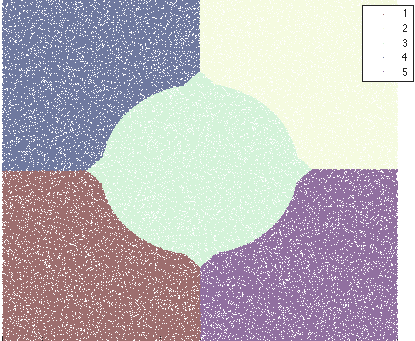
\includegraphics[width=2.3cm]{Ekmeans5.png}}}&
\bmvaHangBox{\fbox{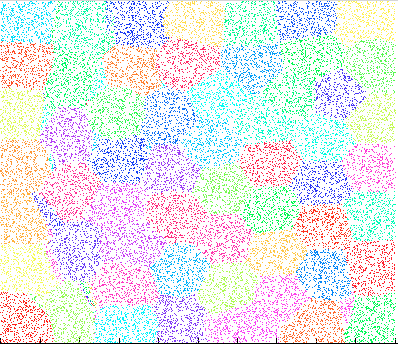
\includegraphics[width=2.7cm]{Ekmeans57.png}}}\\
(a)&(b)
\end{tabular}
\caption{Applying our Assign and Balance variant of Kmeans on 300,000 random 2D points: (a) 5 clusters; (b)  57 clusters (best seen in color).}
\label{fig:ekmeans}
%\label{fig:teaser}
\end{wrapfigure}}

\begin{figure}[t!]
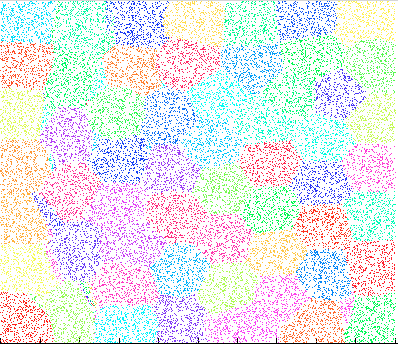
\includegraphics[width=0.45\textwidth]{Ekmeans57.png}
\caption{AB-EKmeans on 300,000 2D points, K= 57}
\label{figABkmeans57}
\end{figure}

Let us denote the set of underfull clusters by $\tilde{C} = \{C_p: |C_p| < N/K \} $. We compute the distances $d(\mathbf{x}_i, \boldsymbol{\mu}_j), \forall \mathbf{x_i} \in \tilde{X} \, \text{and}\, C_i \in \tilde{C}$. Iteratively, we pick the minimum distance pair $(\mathbf{x}_p,\boldsymbol{\mu}_l) $ and assign $\mathbf{x}_p$ to cluster $C_l$ instead of cluster $C(\mathbf{x}_p)$. The point is then removed from the overfull pool. Once an underfull cluster becomes full it is removed from the underfull pool, once an overfull cluster is balanced, the remaining points of that cluster are removed from overfull pool. The intuition behind this algorithms is that,  the cost associated with the initial optimal assignment (given the computed means) is minimally increased by each swap since we pick the minimum distance pair in each iteration. Hence the cost is kept as low as possible while balancing the clusters. We denote the the name of this Algoirthm as Assign and Balance EKmeans. Algorithm~\ref{alg:ddclusterALg1} illustrates the overall assignment step and Fig.~\ref{fig_ABKmeans_balancing} visualizes the balancing step.

\begin{figure} [t!]
\centering
%\centering
%\begin{tabular}{cc}
%\bmvaHangBox{\fbox{
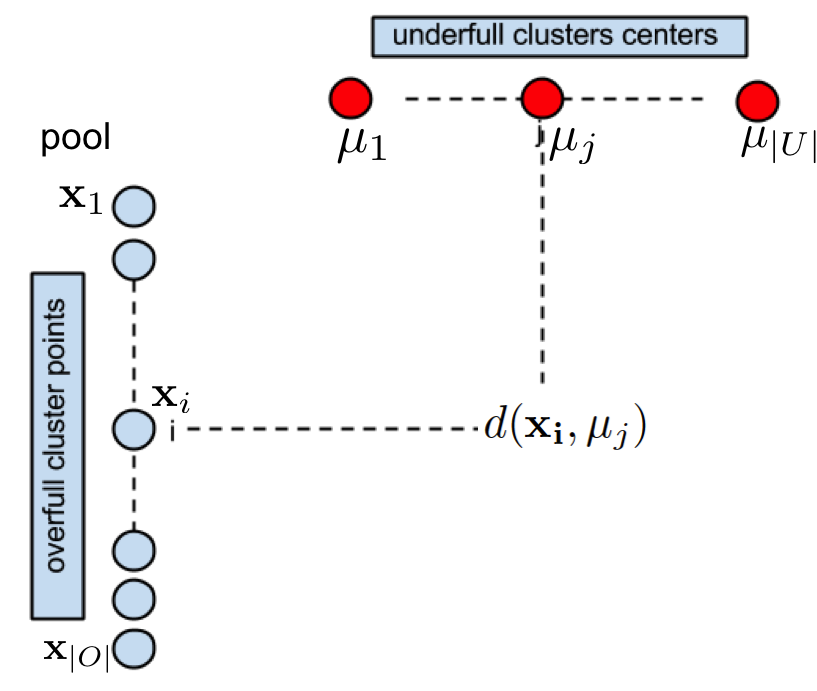
\includegraphics[width=0.40\textwidth]{ABkmeans.png}
\caption{AB Kmeans: Balancing Step}
\label{fig_ABKmeans_balancing}
%\vspace{-3mm}
\end{figure}

\begin{algorithm}[t!]
\KwIn{$\textbf{X} (N \times d_x ),{\{\boldsymbol{\mu}_i\}}_{i=1}^{K}$}
\KwOut{labels}
1- Assign the points initially to its closest center; this will put the clusters into 3 groups (1) balanced clusters   (2) overflowed clusters (3) under-flowed clusters.\\
2- Create a matrix $\textbf{D} \in R^{N \times K}$, where $\textbf{D}[i,j]$ is the distance between the $i^{th}$ point to the $j^{th}$ cluster center; rows are restricted points belongs only to the overflowed clusters; columns are restricted to underflowed cluster centers \\
3- Get the coordinate $(i_*,j_*)$ that maps the smallest distance in $\textbf{D}$.\\
4- Remove the $i_*^{th}$ row from matrix $\textbf{D}$ and mark it as assigned to the $j^{th}$ cluster\\
5- If the size of the cluster $j$ achieves the ideal size (i.e. ~ $n/K$), then remove the $j^{th}$ column from matrix $\textbf{D}$.\\
6- Go to step 3 if there is still unassigned points
\caption{Assign and Balance (AB) k-means: Assignment Step}
\label{alg:ddclusterALg1}
\end{algorithm}


\ignore{
We performed experiments on synthetic datasets (see section ~\ref{sec:6}) on the two proposed variants of k-means algorithms and found that the Assign and Balance algorithm outperform the Iterative Assignment algorithm. Therefore, we focused on RPC and the Assign and Balance algorithm as a pre-processing step for generating the overlapping subdomains. Figure ~\ref{fig:ekmeans} shows example output of the  Assign and Balance algorithm  for assignment on random 2D points. We attach the pseudo-code of the two algorithms in the supplementary materials.}







%Given the input points $\textbf{X} (N \times d_x)$, we decompose them into $K$ clusters. Clusters are denoted as ${\{C_i\}}_{i=1}^{K}$ while the cluster centers are denoted as ${\{\boldsymbol{\mu}_i\}}_{i=1}^{K}$. We also define $|C_i|$ as the number of points in cluster $C_i$. Since we are using clustering to decompose the domain of the training data, Equal size-clusters are more convenient for our purpose  because we are dealing with a regression problem whose performance is affected by the number of points involved in each of the overlapping subdomains (defined later based on the generated clusters). While, there are existing algorithms to deal with size constraints in clustering \cite{Zhu2010}, they are not computationally efficient in practice, epecially for large scale datasets (e.g. Human3.6M ) . This motivates us to propose a variant of kmeans clustering with equal size constraints for the purpose of domain decomposition. The $M$ step (i.e.  computation of the means) in our proposed algorithm is exactly the same as standard kmeans. However, the $E$ (i.e. assignment) step in our algorithm tries to assign the training points, such that the clusters are equal size and the clusters are spatially cohesive as possible. Algorithm ~\ref{alg:ddclusterALg1} and ~\ref{alg:ddclusterALg2} presents two strategies, we implemented to achieve equal size assignment.

\begin{comment}

\begin{algorithm}
\KwIn{$\textbf{X} (N \times d_x ),{\{\boldsymbol{\mu}_i\}}_{i=1}^{K}$}
\KwOut{labels}
1- Assign the points initially to its closest center; this will put the clusters into 3 groups (1) balanced clusters   (2) overflowed clusters (3) under-flowed clusters.\\
2- Create a matrix $\textbf{D} \in R^{N \times K}$, where $\textbf{D}[i,j]$ is the distance between the $i^{th}$ point to the $j^{th}$ cluster center; rows are restricted points belongs only to the overflowed clusters; columns are restricted to underflowed cluster centers \\
3- Get the coordinate $(i_*,j_*)$ that maps the smallest distance in $\textbf{D}$.\\
4- Remove the $i_*^{th}$ row from matrix $\textbf{D}$ and mark it as assigned to the $j^{th}$ cluster\\
5- If the size of the cluster $j$ achieves the ideal size (i.e. ~ $n/K$), then remove the $j^{th}$ column from matrix $\textbf{D}$.\\
6- Go to step 3 if there is still unassigned points
\caption{Equal Size Assignment 1}
\label{alg:ddclusterALg1}
\end{algorithm}


\begin{algorithm}
\KwIn{$\textbf{X} (N \times d_x ),{\{\boldsymbol{\mu}_i\}}_{i=1}^{K}$}
\KwOut{labels}
1- Create a matrix $\textbf{D} \in R^{N \times K}$, where $\textbf{D}[i,j]$ is the distance between the $i^{th}$ point to the $j^{th}$ cluster center.\\
2- Get the coordinate $(i_*,j_*)$ that maps the smallest distance in $\textbf{D}$.\\
3- Remove the $i_*^{th}$ row from matrix $\textbf{D}$ and mark it as assigned to the $j^{th}$ cluster\\
4- If the size of the cluster $j$ achieves the ideal size (i.e. ~ $n/K$), then remove the $j^{th}$ column from matrix $\textbf{D}$.\\
5- Go to step 2 if there is still unassigned points
\caption{Equal Size Assignment 2}
\label{alg:ddclusterALg2}
\end{algorithm}
\end{comment}

\begin{comment}
Algorithm ~\ref{alg:ddclusterALg1} initializes the assignment by applying the $E$ step of the standard kmeans in step 1. Then, the following procedures tries to balance the clusters by transferring points from overflowed clusters (i.e. $|C_i| \succnsim n/NC$) to under-flowed clusters (i.e. $|C_i| \precnsim  n/NC$ ). In algorithm ~\ref{alg:ddclusterALg2}, all points are initially unassigned. Having, distances between all the points and the cluster centers are computed (i.e. $\textbf{D} \in R^{N \times K}$), the point with smallest distance to any of the unfilled clusters is selected ans assigned to the corresponding cluster\footnote{Clusters is marked as filled  when it is assigned to number of points $\approx N/K$}. This process is repeated  until all points are assigned. In order to measure spatial coherency of both Algorithm ~\ref{alg:ddclusterALg1} and ~\ref{alg:ddclusterALg2}, we used the intra-cluster distance measure, given in equation ~\ref{eq:kmeansk}.

\begin{equation}
\begin{split}
{intra}  = \frac 1 N \sum_{i=1}^K \sum_{\textbf{x} \in C_i} {||\textbf{x}-\boldsymbol{\mu}_i||}^2  ,
\end{split} 
\label{eq:kmeansk}
\end{equation}


where $\boldsymbol{\mu}_i$  are  centers of cluster $C_i$.\ignore{ In practice, we found that Algorithm ~\ref{alg:ddclusterALg1} generates more spatially coherent clusters, measured by equation ~\ref{eq:kmeansk}}. We performed some experiments on synthetic datasets (see section ~\ref{sec:6}), we found that Algorithm ~\ref{alg:ddclusterALg1} is better Algorithm ~\ref{alg:ddclusterALg2} using ${intra}$ measure. Hence, we used Algorithm ~\ref{alg:ddclusterALg1} for this pre-processing step. We leave the theoretical analysis of these algorithms as a future work since the main purpose of them is disjoint domain decomposition with spatial coherency.  Figure ~\ref{fig:ekmeans} shows example output of our variant of kmeans with Algorithm ~\ref{alg:ddclusterALg2} for assignment on random 2D points

\end{comment}

\begin{comment}
\begin{figure}
\begin{tabular}{ccc}
\bmvaHangBox{\fbox{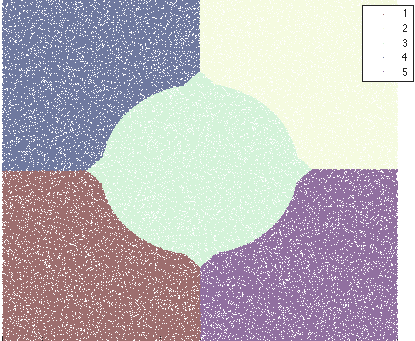
\includegraphics[width=2.3cm]{Ekmeans5.png}}}&
\bmvaHangBox{\fbox{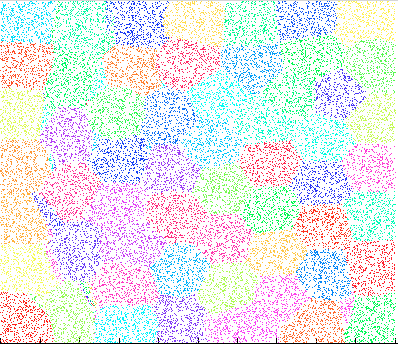
\includegraphics[width=2.7cm]{Ekmeans57.png}}}\\
(a)&(b)
\end{tabular}
\caption{Applying our Assign and Balance variant of Kmeans on 300,000 random 2D points: (a) 5 clusters; (b)  57 clusters.}
\label{fig:ekmeans}
%\label{fig:teaser}
\end{figure}
\end{comment}







%\begin{figure}[h!]
%\centering
%\begin{subfigure}[b]{0.23\textwidth}
%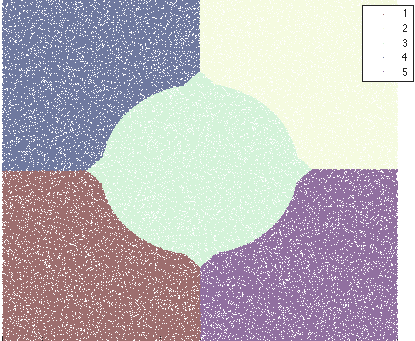
\includegraphics[width=0.99\textwidth]{Ekmeans5}
%\caption{5 clusters}
%\end{subfigure}%
%\begin{subfigure}[b]{0.23\textwidth}
%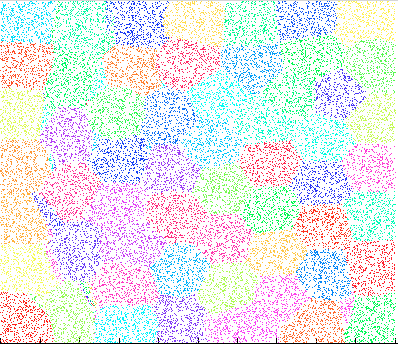
\includegraphics[width=0.99\textwidth]{Ekmeans57}
%\caption{57 clusters}
%\end{subfigure}
%\caption{Applying our Assign and Balance variant of Kmeans on 300,000 random 2D points}
%\label{fig:ekmeans}
%\end{figure}%


\begin{comment}
\begin{algorithm}
\KwIn{$X (N dimes d_x ) , centers (K \times d_x), K$}
\KwOut{labels}
$idealSz =  \frac{n}{K}$ \\
$initLabels = kmeansAssignment(X, centers, K)$ \\
\%  Initialize the labels by the regular kmeans assignment (each point is assigned to the closest center
currSizes $K \time 1$ is the current size of each cluster \\
$OFClusters = the\,clusters\, with\, size > idealSz$ \\
$UFClusters = the\, clusters\, with\, size < idealSz$\\  
$OFCLSz  =$  are the number of points in each of  $OFClusters$ \\
$UFCLSz  =$  are the number of points in each of  $OFClusters$ \\
$OFCLShift (>0)  = OFCLSz - idealSz$  \\
$UFCLShift (<0) = UFCLSz- idealSz$  \\ 
\% Note here that $\sum(OFCLShift(i)) = -\sum(UFCLShift)$
$ActivePts  (NAct \times d_x) = \{x_i \}$ such that $x_i \in  OFClusters$\\
$ActiveUFClusters =  UFClusters$, $NActUF =$ number of ActiveUFClusters \\
$NIter  = sum(OFCLShift(i)) $ \\
$currD  (NAct \times  NActUF ) $ is the distance between all active points and the centers of ActiveUFClusters \\
\For{i=1: NIter}{ $M_i.SubDomain = D_k $  \\
$M_i.K_X =  (K_X)_K $ \\
\% where $(K_X)_K$ is the input kenel matrix evaluated on the points of  $D_k$ only. \\
$M_j.K_Y =  (K_Y)_K $\\
\% where $(K_Y)_K$ is the output kenel matrix evaluated on the points of  $D_k$ only. \\
$M_i.{{K_X}_{inv}} =( K_X + \lambda_x I)^{-1}$ \\
$M_i.{{K_Y}_{inv}} =( K_Y + \lambda_y I)^{-1}$ \\
$M_i.{{\boldsymbol{\mu}_D}_X} =\boldsymbol{\mu}_{D_i}$ \Comment{$d_x \times 1 $ vector}\\ 
$M_i.{{\Sigma_D}_X}^{-1} = {{{\Sigma}_D}_i}^{-1} $  \Comment{$d_x \times d_x $ matrix} \\
\Comment{where $\boldsymbol{\mu}_{D_i}, {{{\Sigma}_D}_i}$ are the MLE estimate mean and covariance estimate for input points in $D_i$ }\\
$DDModel.Models[i] = M_i$;
}
\caption{Equal Size Assignment}
\label{alg:ddtgpm}
\end{algorithm}

Figure ~\ref{fig:ekmeans} shows example output of our variant of kmeans on random 2D points. In order to check the performance of this variant of kmeans on our datasets (high dimensional hog features),  the hog features and cluster labels are fed into $SVM$ with squared exponential kernel $k(x,x') = exp(\frac{x-x'}{{\sigma_x}^2})$ and then we evaluate the accuracy of it like a multiclassification problem to check spatial cohesion.   This algorithm were experimentally tested on POSER, Human Eva, and Human3.6M datasets and they performed well (i.e. all of them give $>98\%$ in this spatial cohesion test). However, we choose to evaluate the generalization of this algorithm as a future work. The purpose here is to create spatially cohesive clusters with equal size which is achieved on the dataset we utilized in our experiment.
\end{comment}
\begin{comment}
\begin{figure}[ht!]
        \centering
        \begin{subfigure}[b]{0.1\textwidth}
                \centering
                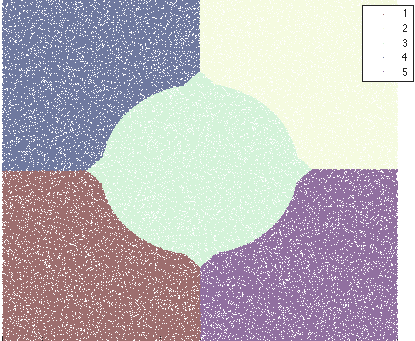
\includegraphics[width=0.8\textwidth]{Ekmeans5}
                \caption{5 clusters}
                \label{fig:ekmeans5}
        \end{subfigure}%
        ~ %add desired spacing between images, e. g. ~, \quad, \qquad etc.
          %(or a blank line to force the subfigure onto a new line)
        \begin{subfigure}[b]{0.1\textwidth}
                \centering
                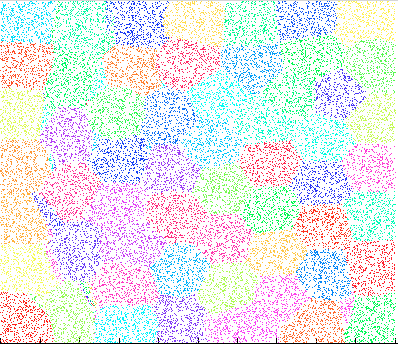
\includegraphics[width=0.8\textwidth]{Ekmeans57}
                \caption{57 clusters}
                \label{fig:ekmeans5}
        \end{subfigure}
        \caption{Equal Size Clustering of 300,000 random 2D points}\label{fig:ekmeans}
\end{figure}
\end{comment}

\vspace{-1.5mm}
\subsubsection{Overlapping Domain Cover(ODC) Model}
\label{sec:train1}

 Having generated the disjoint equal size clusters, we generate the ODC subdomains based on the overlapping ratio $p$, such that $p \cdot M$ points are selected from the neighboring clusters. Let's assume that we select only the closest $r$  clusters to each cluster,  $C_i$ is closer to $C_j$ than $C_k$ if $\| \boldsymbol{\mu}_i - \boldsymbol{\mu}_j\| < \| \boldsymbol{\mu}_i - \boldsymbol{\mu}_k\|$. It is important to note that $r$ must be greater than  $p/(1-p)$ in order to supply the required $p \cdot M$ points; this is since number of points in each cluster is $(1-p) M$. Hence, the minimum value for $r$ is $\lceil(p \cdot M)/ ( (1-p)  \cdot M)\rceil = \lceil p/(1-p) \rceil$ clusters. Hence, we parametrize $r$ as $r =  \lceil t \cdot p/(1-p) \rceil, t\ge 1$. We study the effect of $t$ in the experimental results section. Having computed $r$ from $p$ and $t$, each subdomain $D_i$ is then created by merging the points in the cluster $C_i$ with $p \cdot M$ points, retrieved from the $r$ neighboring clusters. Specifically, the points are selected by sorting the points in each of $r$ clusters by the distance to $\boldsymbol{\mu}_i$. The number of points retrieved for each of the $r$ neighboring clusters is inversely proportional to the distance of its center to $\boldsymbol{\mu}_i$. If a subset of the $r$ clusters are requested to retrieve more than its capacity (i.e., $(1-p) M$), the set of the extra points are requested from the remaining clusters giving priority to the closer clusters (i.e., starting from the nearest neighboring cluster to the cluster on which the subdomain is created). \ignore{Its is worth to mention that a}As $t=1$ and $p$ increases, all points that belong to the $r$ clusters tends to be merged with $C_i$. In our framework, we used FLANN ~\cite{flann09} for fast NN-retrieval; see pseudo-code of ODC generation in  Appendix C.
 \ignore{
 ????? Does it need a clarification or an example ????.  
 We constraint these points to belong to up to $r$ clusters. If they belong to more than $r$ clusters, The closest clusters are chosen based on the distance between the cluster centers (i.e.  $\|\ \boldsymbol{\mu}_i - \boldsymbol{\mu}_j\|\, j=1:K , j \neq i$ ). Since, $|C_i| \approx N / K$ for equal size clusters, we choose $r \ge b \cdot K / N$, to guarantee that that there is at least $b$ points in the neighboring $r$ clusters. Hence, we define number of points in each subdomain as $M \approx N / K + b$. A successful assignment from our experiments is to increase $b$ with respect to $N/K$. We attach a detailed prescription of the parameter selection and the pseudo-code of the our Overlapping Domain Cover algorithm  and implementation details in the supplementary materials.}
 
\begin{comment}
\begin{algorithm}
{\textbf{Input:} Clusters ${\{C_k\}}_{k=1}^{K} $}
\KwOut{Overlapping subdomains ${\{D_k\}}_{k=1}^{K}$}
\ForEach{Cluster $C_k$}{
Compute the closest $OCC$ clusters ${\{{{OVC_K}_i}\}}_{i=1}^{OCC}$ based on $DK_i = \| \boldsymbol{\mu}_k- \boldsymbol{\mu}_i \|$ , $i\neq k$\\
Let $LK_i = 1/DK_i,  {WK_i} =  \frac{LK_i}{\sum_{l=1}^{OCC} LK_l}$  ${i=1 : OCC}$\\
Let ${NPK_i} =  floor(WK_i * OPC)$, ${i=1 : OCC}$ \\
Let $ExKPts = OPC - \sum_{l=1}^{OCC} NPK_l$ \\
Let ${NPK_i}$ =  $NPK_i +1$ , $ i=1 : ExKPts $\\
$D_k =  C_k$ \\
\For{i=1 : OCC} { $Ps_i = KNN({OVC_K}_j,NPK_i )$ \\ $D_k = D_k \cup Ps_i$ }

\Comment{where KNN is the K-nearest neighbors algorithms. For high performance calculation of $KNN$, we use FLANN \cite{flann09} to calculate $KNN$.}
}
\caption{Subdomains Generation (Note: All ${\{D_k\}}_{k=1}^{K}$ are stored as indices to $X$).  }
\label{alg:sdgen}
\end{algorithm}
\end{comment}

%\vspace{-1mm}
%\subsection{ODCModel Generation}
%\label{sec:train2}

\ignore{Having generated the ODC,}After the ODC is generated, we compute the the sample normal distribution using the points that belong to each subdomain. Then, a local kernel machine is trained for each of the overlapping subdomains. We denote the point set normal distribution of the subdomains as $p(\mathbf{x}|D_i) = \mathcal{N}(\boldsymbol{\mu}'_i \in R^{d_X}, \Sigma'_i \in R^{d_X \times d_X})$;\ignore{
\begin{equation}
p(\mathbf{x}|D_i) = \mathcal{N}(\boldsymbol{\mu}'_i \in R^{d_x}, \Sigma'_i \in R^{d_x \times d_x})
\end{equation}}
 ${\Sigma'}_i^{-1}$ is precomputed during the training for later use during the prediction. \ignore{The main rationale behind using our overlapping subdomain notion, is} Finally, we factor out all the computations that does not depend on the test point (for GPR, TGP, IWTGP) and store them with each sub domain as its local kernel machine. We denote the training model for subdomain $i$ as $\mathcal{M}^i$, which is computed as follows for GPR and TGP respectively.%; see SM for IWTGP.
\ignore{
foot  IWTGP respectively.}


\textbf{ {GPR}.}\ignore{In order to compute $\mathcal{M}^i$ In the case of GPR, we first precompute $(\textbf{K}^i_j + \sigma^2_{n^i_j} \textbf{I})^{-1} $, where  $\textbf{K}^i_j$ is an $M \times M$  kernel matrix, defined on the input points that belong to domain $i$. Since, GPR does not capture dependency between output dimensions, each dimension $j$ in the output could have its own hyper-parameters, which results in a different kernel matrix for each dimension $\textbf{K}^i_j$. We also precompute $(\textbf{K}^i_j + \sigma^2_{n^i_j} \textbf{I})^{-1} \textbf{y}_j$ for each dimension. Hence  $\mathcal{M}^i = \{ ( \textbf{K}^i_j + \sigma^2_{n^i_j} \textbf{I})^{-1},  (\textbf{K}^i_j + \sigma^2_{n^i_j} \textbf{I})^{-1} \textbf{y}_j ), j=1 : d_Y \}$.} Firstly, we  precompute $(\textbf{K}^i_j + \sigma^2_{n^i_j} \textbf{I})^{-1} $, where  $\textbf{K}^i_j\,$ is an $M \times M\,$  kernel matrix, defined on the input points in  $D_i$. Each dimension $j$ in the output could have its own hyper-parameters, which results in a different kernel matrix for each dimension $\textbf{K}^i_j$. We also precompute $(\textbf{K}^i_j + \sigma^2_{n^i_j} \textbf{I})^{-1} \textbf{y}_j$ for each dimension. Hence  $\mathcal{M}^i_{GPR} = \small\{ ( \textbf{K}^i_j + \sigma^2_{n^i_j} \textbf{I})^{-1},  (\textbf{K}^i_j + \sigma^2_{n^i_j} \textbf{I})^{-1} \textbf{y}_j )$ $, j=1 : d_Y \}\normalsize$.

\textbf{{TGP.}} \ignore{Since, TGP captures the the dependency between the outputs, t } The local kernel machine for each subdomain in TGP case is defined as $\mathcal{M}^i_{TGP} = \small\{(\textbf{K}_X^i + \lambda_{X}^i  \textbf{I})^{-1}, (\textbf{K}_Y^i + \lambda_{Y}^i  \textbf{I})^{-1}\}\normalsize$,  where $\textbf{K}_X^i$ and $\textbf{K}_Y^i$ are $M \times M$ kernel matrices defined on the input points and the corresponding output points respectively, which belong to domain $i$. 


\textbf{IWTGP. } It is not obvious how to factor out computations that does not depend on the test data in the case of IWTGP, since the computational extensive factor(i.e., $({\textbf{W}^i}^\frac{1}{2} $ $\textbf{K}_X^i {\textbf{W}^i}^\frac{1}{2} + \lambda_x^i \textbf{I})^{-1}$,  $({\textbf{W}^i}^\frac{1}{2} \textbf{K}_Y^i {\textbf{W}^i}^\frac{1}{2} + \lambda_y^i \textbf{I})^{-1}$ ) does depend on the test set since $\textbf{W}^i$ is computed on test time.  To help factor out the computation, we used linear algebra to show that
\begin{equation}
(\textbf{D A D} + \lambda \textbf{I})^{-1} =   \textbf{D}^{-1} \textbf{A}^{-1} \textbf{D}^{-1} - \frac{\lambda \textbf{D}^{-2} \textbf{A}^{-2} \textbf{D}^{-2}} {1 + \lambda \cdot  tr(\textbf{D}^{-1} \textbf{A}^{-1} \textbf{D}^{-1})}
\label{eq:lem}
\end{equation}
where $\textbf{D}$ is a diagonal matrix,  $I$ is the identity matrix, and $tr(\textbf{B})$ is the trace of matrix $\textbf{B}$.  \begin{proof}
Kenneth Miller~\cite{Miller1981} proposed the following Lemma on Matrix Inverse. 
 \begin{equation}
 (G+H)^{-1} = G^{-1} -\frac{1}{1+tr(G H^{-1})} G^{-1} H G^{-1} 
 \end{equation}
  Applying Miller's lemma, where  $G = D A D$ and $H = \lambda I$, leads directly to Eq.~\ref{eq:lem}. %$(\textbf{D A D} + \lambda \textbf{I})^{-1} =   \textbf{D}^{-1} \textbf{A}^{-1} \textbf{D}^{-1} - $ $\frac{\lambda (\textbf{D}^{-1} \textbf{A}^{-1} \textbf{D}^{-1})^{2}} {1 + \lambda^{-1} \cdot  tr(\textbf{D}^{-1} \textbf{A}^{-1} \textbf{D}^{-1})}$.
 \end{proof}
 




Mapping $\textbf{D}$ to ${\textbf{W}^i}^\frac{1}{2}$ \footnote{$\textbf{W}$ is a diagonal matrix}, $\textbf{A}$ to either of $\textbf{K}_X^i$ or $\textbf{K}_Y^i$, we can compute $\mathcal{M}^i = \{{\textbf{K}_X^i}^{-1}, {\textbf{K}_Y^i}^{-1}\}$. Having computed $\textbf{W}^i$ on test time,  $({\textbf{W}^i}^\frac{1}{2} \textbf{K}_X^i {\textbf{W}^i}^\frac{1}{2} + \lambda_x \textbf{I})^{-1}$,  $({{\textbf{W}^i}}^\frac{1}{2} \textbf{K}_X {\textbf{W}^i}^\frac{1}{2} + \lambda_x \textbf{I})^{-1}$ could be computed in quadratic time given  $\mathcal{M}^i$  following equation ~\ref{eq:lem}, since the inverse and the power of ${\textbf{W}^i}^\frac{1}{2}$ has linear computational complexity since it is diagonal. 

%\section{Proof that $(\textbf{D A D} + \lambda \textbf{I})^{-1} =   \textbf{D}^{-1} \textbf{A}^{-1} \textbf{D}^{-1} - \frac{\lambda(\textbf{D}^{-1} \textbf{A}^{-1} \textbf{D}^{-1})^{2}} {1 + \lambda^{-1} \cdot  tr(\textbf{D}^{-1} \textbf{A}^{-1} \textbf{D}^{-1})}$}

%\textbf{Proof that $(\textbf{D A D} + \lambda \textbf{I})^{-1} =   \textbf{D}^{-1} \textbf{A}^{-1} \textbf{D}^{-1} - $ $\frac{\lambda(\textbf{D}^{-1} \textbf{A}^{-1} \textbf{D}^{-1})^{2}} {1 + \lambda^{-1} \cdot  tr(\textbf{D}^{-1} \textbf{A}^{-1} \textbf{D}^{-1})}$ : }

\begin{comment}
\textbf{ITWTGP (sec ~\ref{ss:cstgp}) :} It is not obvious how to factor out computations that does not depend on the test data in the case of IWTGP, since the computational extensive factor(i.e. $({\textbf{W}^i}^\frac{1}{2} \textbf{K}_X^i {\textbf{W}^i}^\frac{1}{2} + \lambda_x^i \textbf{I})^{-1}$,  $({\textbf{W}^i}^\frac{1}{2} \textbf{K}_Y^i {\textbf{W}^i}^\frac{1}{2} + \lambda_y^i \textbf{I})^{-1}$ ) does depend on the test set since $\textbf{W}^i$ is computed on test time. However, we utilized the following theorem from linear algebra to help us factor out the computation; proof is attached in the supplementary materials.
\begin{equation}
(\textbf{D A D} + \lambda \textbf{I})^{-1} =   \textbf{D}^{-1} \textbf{A}^{-1} \textbf{D}^{-1} - \frac{\lambda \textbf{D}^{-2} \textbf{A}^{-2} \textbf{D}^{-2}} {1 + \lambda \cdot  tr(\textbf{D}^{-1} \textbf{A}^{-1} \textbf{D}^{-1})}
\label{eq:lem}
\end{equation}

, where $\textbf{D}$ is a diagonal matrix,  $I$ is the identity matrix, and $tr(\textbf{B})$ is the trace of matrix $\textbf{B}$. Mapping $\textbf{D}$ to ${\textbf{W}^i}^\frac{1}{2}$ \footnote{$\textbf{W}$ is a diagonal matrix}, $\textbf{A}$ to either of $\textbf{K}_X^i$ or $\textbf{K}_Y^i$, we can compute $\mathcal{M}^i = \{{\textbf{K}_X^i}^{-1}, {\textbf{K}_Y^i}^{-1}\}$. Having computed $\textbf{W}^i$ on test time,  $({\textbf{W}^i}^\frac{1}{2} \textbf{K}_X^i {\textbf{W}^i}^\frac{1}{2} + \lambda_x \textbf{I})^{-1}$,  $({{\textbf{W}^i}}^\frac{1}{2} \textbf{K}_X {\textbf{W}^i}^\frac{1}{2} + \lambda_x \textbf{I})^{-1}$ could be computed in quadratic time given  $\mathcal{M}^i$  following equation ~\ref{eq:lem}, since the inverse and the power of ${\textbf{W}^i}^\frac{1}{2}$ has linear computational complexity. .

\end{comment}

\ignore{ information are created and stored in DDTGP model as illustrated in Algorithm ~\ref{alg:ddtgpm}.
\begin{algorithm}
{\textbf{Input:} Clusters ${\{C_k\}}_{k=1}^{NC} $}
\KwOut{Overlapping subdomains ${\{D_k\}}_{k=1}^{NC}$}
\ForEach{Cluster $C_k$}{
Compute the closest $OCC$ clusters ${\{{{OVC_K}_i}\}}_{i=1}^{OCC}$ based on $DK_i = \| \boldsymbol{\mu}_k- \boldsymbol{\mu}_i \|$ , $i\neq k$\\
Let $LK_i = 1/DK_i,  {WK_i} =  \frac{LK_i}{\sum_{l=1}^{OCC} LK_l}$  ${i=1 : OCC}$\\
Let ${NPK_i} =  floor(WK_i * OPC)$, ${i=1 : OCC}$ \\
Let $ExKPts = OPC - \sum_{l=1}^{OCC} NPK_l$ \\
Let ${NPK_i}$ =  $NPK_i +1$ , $ i=1 : ExKPts $\\
$D_k =  C_k$ \\
\For{i=1 : OCC} { $Ps_i = KNN({OVC_K}_j,NPK_i )$ \\ $D_k = D_k \cup Ps_i$ }
}
\Comment{where KNN is the K-nearest neighbors algorithms. For high performance calculation of $KNN$, we use FLANN \cite{flann09} to calculate $KNN$.}
\caption{Subdomains Generation (Note: All ${\{D_k\}}_{k=1}^{NC}$ are stored as indices to $X$).  }
\label{alg:sd}
\end{algorithm}}


\begin{comment}
\begin{algorithm}
\KwIn{Overlapping subdomains ${\{D_k\}}_{k=1}^{NC}$}
\KwOut{DDModel (Domain Decomposition TGP Model) }
\For{i=1: NC}{ $M_i.SubDomain = D_k $  \\
$M_i.K_X =  (K_X)_K $ \\
\% where $(K_X)_K$ is the input kenel matrix evaluated on the points of  $D_k$ only. \\
$M_j.K_Y =  (K_Y)_K $\\
\% where $(K_Y)_K$ is the output kenel matrix evaluated on the points of  $D_k$ only. \\
$M_i.{{K_X}_{inv}} =( K_X + \lambda_x I)^{-1}$ \\
$M_i.{{K_Y}_{inv}} =( K_Y + \lambda_y I)^{-1}$ \\
$M_i.{{\boldsymbol{\mu}_D}_X} =\boldsymbol{\mu}_{D_i}$ \Comment{$d_x \times 1 $ vector}\\ 
$M_i.{{\Sigma_D}_X}^{-1} = {{{\Sigma}_D}_i}^{-1} $  \Comment{$d_x \times d_x $ matrix} \\
\Comment{where $\boldsymbol{\mu}_{D_i}, {{{\Sigma}_D}_i}$ are the MLE estimate mean and covariance estimate for input points in $D_i$ }\\
$DDModel.Models[i] = M_i$;
}
\caption{DDTGP Model Generation}
\label{alg:ddtgpm}
\end{algorithm}
\end{comment}
\ignore{
\begin{algorithm}
\KwIn{Overlapping subdomains ${\{D_k\}}_{k=1}^{NC}$}
\KwOut{DDModel (Domain Decomposition TGP Model) }
\For{i=1: NC}{ $M_i.SubDomain = D_k $  \\
$M_i.K_X =  (K_X)_k $ \\
\% where $(K_X)_k$ is the input kenel matrix evaluated on the points of  $D_k$ only. \\
$M_j.K_Y =  (K_Y)_k $\\
\% where $(K_Y)_k$ is the output kenel matrix evaluated on the points of  $D_k$ only. \\
$M_i.{{K_X}_{inv}} =( M_i.K_X + \lambda_x I)^{-1}$ \\
$M_i.{{K_Y}_{inv}} =( M_i.K_Y + \lambda_y I)^{-1}$ \\
$M_i.{{\boldsymbol{\mu}_D}_X} =\boldsymbol{\mu}_{D_i}$ \Comment{$d_x \times 1 $ vector}\\ 
$M_i.{{\Sigma_D}_X}^{-1} = {{{\Sigma}_D}_i}^{-1} $  \Comment{$d_x \times d_x $ matrix} \\
\Comment{where $\boldsymbol{\mu}_{D_i}, {{{\Sigma}_D}_i}$ are the MLE estimate mean and covariance estimate for input points in $D_i$ (used in Mode 3) }\\
$DDModel.Models[i] = M_i$;
}
\caption{DDTGP Model Generation}
\label{alg:ddtgpm}
\end{algorithm}
}
\ignore{
\begin{algorithm}
\KwIn{query point X, DDTGPModel}
\KwOut{Closest subdomains }
Let $KNN_x =  KNN(x, X)$  \Comment{X is all input training points.} \\
Let ${L_{KNN_x}} =  Clusters(KNN_x)$ \Comment{where Clusters($KNN_x$) returns the corresponding clusters for the returned points.} \\ 
$FT = frequencyTable(L_{KNN_x})$ \Comment{where $frequencyTable(L_{KNN_x})$ returns an frequency of each clusters in $L_{KNN_x}$. }\\
$[sortedFT, sortedInd]  = sort(FT$) \\
$closestDomains = sortedInd[1:CDC] $\\ 
$closestFTS = sortedFT[1:CDC]$ \\
\caption{Mode 2 closest clusters algorithm}
\label{alg:mode2FC}
\end{algorithm}
}
\begin{comment}

\begin{figure}[h!]
  \null\hfill \algTwo{alg2} \hfill \algThree{alg3} \hfill\null\par 
\end{figure}
\end{comment}



